
\documentclass[journal]{IEEEtran}
%
% If IEEEtran.cls has not been installed into the LaTeX system files,
% manually specify the path to it like:
% \documentclass[journal]{../sty/IEEEtran}
\usepackage{graphicx}
\usepackage{xcolor}
\usepackage{soul}
\usepackage{url}
\usepackage{comment}
\usepackage{longtable}
\usepackage{enumitem}
\usepackage{cite}
\usepackage{listings}
\usepackage{amsmath,amssymb,amsthm}
\usepackage{booktabs}
\graphicspath{{figs/}}


% *** GRAPHICS RELATED PACKAGES ***
%
\ifCLASSINFOpdf
  % \usepackage[pdftex]{graphicx}
  % declare the path(s) where your graphic files are
  % \graphicspath{{../pdf/}{../jpeg/}}
  % and their extensions so you won't have to specify these with
  % every instance of \includegraphics
  % \DeclareGraphicsExtensions{.pdf,.jpeg,.png}
\else
  % or other class option (dvipsone, dvipdf, if not using dvips). graphicx
  % will default to the driver specified in the system graphics.cfg if no
  % driver is specified.
  % \usepackage[dvips]{graphicx}
  % declare the path(s) where your graphic files are
  % \graphicspath{{../eps/}}
  % and their extensions so you won't have to specify these with
  % every instance of \includegraphics
  % \DeclareGraphicsExtensions{.eps}
\fi
% graphicx was written by David Carlisle and Sebastian Rahtz. It is
% required if you want graphics, photos, etc. graphicx.sty is already
% installed on most LaTeX systems. The latest version and documentation
% can be obtained at: 
% http://www.ctan.org/pkg/graphicx
% Another good source of documentation is "Using Imported Graphics in
% LaTeX2e" by Keith Reckdahl which can be found at:
% http://www.ctan.org/pkg/epslatex
%
% latex, and pdflatex in dvi mode, support graphics in encapsulated
% postscript (.eps) format. pdflatex in pdf mode supports graphics
% in .pdf, .jpeg, .png and .mps (metapost) formats. Users should ensure
% that all non-photo figures use a vector format (.eps, .pdf, .mps) and
% not a bitmapped formats (.jpeg, .png). The IEEE frowns on bitmapped formats
% which can result in "jaggedy"/blurry rendering of lines and letters as
% well as large increases in file sizes.
%
% You can find documentation about the pdfTeX application at:
% http://www.tug.org/applications/pdftex



% correct bad hyphenation here
\hyphenation{op-tical net-works semi-conduc-tor}


\begin{document}
%
% paper title
% Titles are generally capitalized except for words such as a, an, and, as,
% at, but, by, for, in, nor, of, on, or, the, to and up, which are usually
% not capitalized unless they are the first or last word of the title.
% Linebreaks \\ can be used within to get better formatting as desired.
% Do not put math or special symbols in the title.
\title{Spatiotemporal Computational Modeling of Cascading Failures for Urban Resilience: A Case Study of Recife}
%
%
% author names and IEEE memberships
% note positions of commas and nonbreaking spaces ( ~ ) LaTeX will not break
% a structure at a ~ so this keeps an author's name from being broken across
% two lines.
% use \thanks{} to gain access to the first footnote area
% a separate \thanks must be used for each paragraph as LaTeX2e's \thanks
% was not built to handle multiple paragraphs
%

\author{Rosiberto~Gonçalves*,
        Ingrid~Lima,
        Isabela~Lima,
        Nicolas~Cajueiro% <-this % stops a space
\thanks{*Rosiberto Gonçalves with the Estácio Recife University, Recife,
PE, Brazil e-mail: (rosibertosantos@gmail.com).}% <-this % stops a space
}




% The paper headers
\markboth{}{R. GONÇALVES et al.: Spatiotemporal Computational Modeling of Cascading}



% make the title area
\maketitle

% As a general rule, do not put math, special symbols or citations
% in the abstract or keywords.
\begin{abstract}
Urban smart systems depend on tightly coupled critical infrastructures. Climate-induced extreme events may trigger cascading failures across energy and telecommunication networks, threatening service continuity. This study proposes a percolation-theory-based resilience framework applied to interdependent urban networks. A novel Urban Resilience Percolation Index (IRU-P) is introduced, integrating structural robustness, temporal recovery dynamics, and critical percolation thresholds. Using geospatial data from Recife (Brazil), we simulate flood-driven cascading failures through Monte Carlo experiments and perform parametric sensitivity analysis. Results demonstrate statistically significant reductions in systemic functionality under spatially concentrated disruptions (p < 0.01), revealing nonlinear vulnerability amplification. The framework provides a decision-support tool aligned with ISO 37123 and SDG 11.
\end{abstract}

% Note that keywords are not normally used for peerreview papers.
\begin{IEEEkeywords}
Urban Resilience, Cascading Failures, Critical Infrastructure, Interdependent Networks, Recife.
\end{IEEEkeywords}






% For peer review papers, you can put extra information on the cover
% page as needed:
% \ifCLASSOPTIONpeerreview
% \begin{center} \bfseries EDICS Category: 3-BBND \end{center}
% \fi
%
% For peerreview papers, this IEEEtran command inserts a page break and
% creates the second title. It will be ignored for other modes.
\IEEEpeerreviewmaketitle



\section{Introduction}
Urban areas increasingly depend on critical infrastructures to provide essential services to the population. Electric power, telecommunications, transportation, water supply, and other urban systems are connected through physical, operational, and digital dependencies~\cite{Wang2026}. These relationships improve the operation of cities but also create conditions in which a failure in one infrastructure can affect other interconnected systems. As a result, a local disruption can develop into a cascading failure and cause service interruptions beyond the initially affected area~\cite{Wang2026,Chowdhury2026}.

Climate-related hazards increase the exposure of urban infrastructures to these disruptions. Heavy rainfall, flooding, and landslides can damage infrastructure components and interrupt essential services. The effects can be amplified when infrastructures depend on each other~\cite{Liu2025}. For example, a failure in the electric power network can affect telecommunications equipment and network availability. In turn, the loss of telecommunications services can impair emergency communication, coordination of public services, and access to information. The analysis of these events therefore requires models that consider the interactions between infrastructure networks rather than evaluating each network independently.

Urban resilience has been used to describe the capacity of urban systems to withstand disruptions and maintain or restore essential services~\cite{Yadav2019}. Several studies have proposed network-based approaches to evaluate the resilience of critical infrastructures. However, the analysis of interdependent networks remains challenging because the effects of a failure depend on the topology of each network, the dependencies between network layers, the location of the affected components, and the propagation mechanisms considered~\cite{Liu2025}. Network degradation can also reach critical points at which the loss of a relatively small number of components produces a significant reduction in network connectivity.

Percolation theory provides a mathematical framework for studying connectivity and structural transitions in complex networks~\cite{Li2021}. In infrastructure networks, percolation models can be used to analyze how the removal of nodes or links affects network connectivity and to identify conditions associated with the loss of a functional connected component. When applied to interdependent networks, this approach also allows the effects of failures in one network to be propagated to dependent components in another network. This makes percolation theory suitable for studying cascading failures and critical conditions in interconnected urban infrastructures.

Recife, Brazil, provides a relevant case for this type of analysis. The city has a dense urban structure, extensive low-lying areas, and recurrent episodes of intense rainfall and flooding. These characteristics expose critical infrastructure to disruptions that can affect essential urban services~\cite{tcepe2024}. The strong dependence between electrical and telecommunications infrastructure also provides an appropriate context for analyzing how localized failures can propagate between network layers.

Despite the existing research on urban resilience, critical infrastructure, and interdependent networks, there is still a need for computational models that combine network structure, interlayer dependencies, failure propagation, and quantitative resilience metrics. In particular, the identification of critical conditions associated with network degradation and systemic collapse requires models that can represent different failure scenarios and measure their effects on network connectivity over time.

This study proposes a computational model for the analysis of cascading failures in interdependent electric power and telecommunications networks, using Recife as a case study. The networks are represented as interconnected graphs, and a percolation-based approach is used to model the propagation of failures between infrastructure layers. The model is implemented in Python using NetworkX~\cite{hagberg2008} and supports random, targeted, and geospatial failure scenarios. The analysis considers metrics such as the percentage of active nodes, the size of the largest connected component, network robustness, and estimated system recovery time.

The proposed model provides a computational framework for evaluating the effects of cascading failures on interdependent urban infrastructures. The use of Recife as a case study allows the model to be evaluated in a specific urban and environmental context, while its computational structure can be adapted to other cities and infrastructure configurations.

The main contributions of this work are:

\begin{enumerate}
\item Integrated methodological framework: The combination of graph theory, percolation theory, and geospatial analysis enables an accurate representation of interdependencies among infrastructures and the spatial correlation of natural disasters.
\item Percolation-Based Urban Resilience Index: The Percolation-Based Urban Resilience Index provides a quantitative, reproducible, and interpretable metric that integrates the structural and dynamic dimensions of resilience, while remaining compatible with international indicators of sustainable cities.
\item Evidence from the Recife case study: The simulations demonstrated that spatially concentrated flooding scenarios produce 37\% greater systemic degradation than random failures, highlighting the city's specific vulnerability to extreme climate events.
\item Replicable computational tool: The model implemented in Python/NetworkX is modular and scalable and can be adapted to other Brazilian and international cities through the replacement of input data (network topology and risk maps).
\end{enumerate}

\section{Literature Review}

The analysis of the robustness of complex networks has been the subject of study since early works on fault and attack tolerance in networks with different topological properties. Albert et al. \cite{albert2000} showed that scale-free networks exhibit high tolerance to random node removal but can be significantly affected by attacks targeting their most connected nodes. These results established a relationship between network topology and its vulnerability to different types of failure. Subsequently, studies extended this analysis to systems formed by interdependent networks. Buldyrev et al. \cite{buldyrev2010} demonstrated that interdependencies between networks can produce abrupt phase transitions and lead to a significant loss of connectivity when the proportion of removed components exceeds certain critical values.

Percolation theory provides a basis for analyzing these transitions and evaluating network connectivity under the removal of nodes or links. In interdependent networks, the problem becomes more complex due to the propagation of failures between different layers. A failure in one network can cause dependent components in another network to become unavailable, initiating an iterative degradation process. This behavior distinguishes interdependent networks from isolated networks and requires consideration of both the individual structure of the networks and the dependency relationships between them \cite{buldyrev2010}.

The application of complex network concepts to the study of urban systems has increased due to the need to represent relationships between different infrastructure components. Newman \cite{newman2018} presents foundations for the analysis of complex networks, including structural properties, connectivity, and degree distribution, which are relevant to the study of network robustness. In the context of critical infrastructures, these properties can be used to identify important components and analyze the effects of removing elements from the network.

Urban infrastructures, however, have characteristics that are not fully represented by models based only on topology. The location of components, the spatial distribution of risks, and the dependencies between different services can influence how a failure propagates. During events such as heavy rainfall, flooding, and landslides, for example, components located in certain areas may have a higher probability of failure. The incorporation of geospatial information therefore allows scenarios to be represented in which the location of components and their exposure to risks are part of the initial failure definition process.

Studies on the resilience of critical infrastructures~\cite{Karakoc2019, Nan2016A, Poulin2021} have also used connectivity, availability, and recovery metrics to evaluate system behavior after disruptive events. These metrics allow different failure scenarios to be compared and changes in the functional capacity of the network to be identified. However, individual metrics may not fully represent the effects of failures propagating across interdependent infrastructures. The combination of network metrics and propagation models can provide a more consistent assessment of systemic degradation.

In the context of resilient cities, ISO 37123~\cite{iso37123} establishes indicators for assessing urban performance and resilience. The standard covers different dimensions related to the ability of cities to deal with risks and service disruptions. Although these indicators are relevant to urban assessment, they do not replace computational models capable of representing the dynamics of failures between interdependent infrastructure components. There is therefore room to relate urban resilience indicators to quantitative models based on network structure and connectivity.

The literature also shows a separation between three aspects that are relevant to the problem investigated in this work. The first concerns the structural robustness of networks and the identification of critical components. The second involves the propagation of failures between interdependent networks. The third considers the spatial dimension of events and the evolution of degradation over time. Integrating these aspects is important for representing situations in which a localized failure can produce systemic effects across different infrastructures.

Based on this literature, this work considers electric power and telecommunications networks as interdependent systems and uses percolation theory to analyze failure propagation and the conditions associated with connectivity degradation. The model also incorporates different strategies for defining initial failures, including random, targeted, and geospatial failures. This approach allows the effects of different failure patterns to be compared and changes in network resilience metrics to be evaluated for each scenario.

\section{Materials and Methods}
This section details the mathematical and computational formulation of the proposed model. The approach integrates complex network theory, percolation theory, and geospatial analysis to simulate the propagation of failures in interdependent critical infrastructures.


\subsection{Interdependent Network Modeling}
The model considers two interdependent infrastructure networks: an electric power network and a telecommunications network. Each network is represented as an undirected graph:

\begin{equation}
G_E = (V_E, E_E), \qquad G_T = (V_T, E_T)
\label{eq:networks}
\end{equation}

where $V_E$ and $V_T$ represent the sets of nodes (e.g., substations and communication towers) in the electric power and telecommunications networks, respectively, while $E_E$ and $E_T$ represent their respective physical or logical connections.

To formalize the interdependence, a coupling network $G_C$ is defined to represent the functional dependencies between the layers. A node $v \in V_E$ is considered a supporting node for a node $u \in V_T$ if the operation of $u$ strictly depends on the power supply provided by $v$. Therefore, the unavailability of a component in one layer may induce the failure of dependent components in the other layer.


The computational implementation of this interlayer coupling is performed using a hybrid algorithm that prioritizes geographical proximity (85\% spatial coupling based on the shortest Euclidean distance) and adds random logical connections (15\%), as implemented in Algorithm \ref{code:coupling}.

\begin{lstlisting}[
    language=Python, 
    caption={Interdependent Coupling Algorithm.}, 
    label=code:coupling,
    basicstyle=\footnotesize\ttfamily, 
    breaklines=true,                   
    columns=fullflexible,              
    keepspaces=true
]
def _build_coupling(self):
    deps = {}
    E_nodes = list(self.G_E.nodes())
    for t in self.G_T.nodes():
        t_pos = (self.G_T.nodes[t]["lon"], self.G_T.nodes[t]["lat"])
        dists = []
        for e in E_nodes:
            e_pos = (self.G_E.nodes[e]["lon"], self.G_E.nodes[e]["lat"])
            d = np.sqrt((t_pos[0] - e_pos[0])**2 + (t_pos[1] - e_pos[1])**2)
            dists.append((e, d))
        if np.random.random() < 0.85:
            dists.sort(key=lambda x: x[1])
            deps[t] = dists[0][0]
        else:
            deps[t] = np.random.choice(E_nodes)
    return deps
\end{lstlisting}


The fraction of active nodes in the system at a given time is defined as:

\begin{equation}
p = \frac{|V_{\mathrm{active}}|}{|V|}
\label{eq:occupation}
\end{equation}


where $|V_{\mathrm{active}}|$ represents the number of functional nodes, and $|V|$ represents the total number of nodes in the interdependent system.

\subsection{Failure Propagation Mechanism and Percolation Threshold}
The propagation of cascading failures is modeled as a discrete iterative process. Initially, a set of nodes is removed, representing the initial shock. At each iteration step $t$, failures propagate through interlayer dependencies and the loss of topological connectivity. The iterative process continues until no further failures occur, reaching the following stability condition:


\begin{equation}
\Delta \left|V_{\mathrm{active}}\right| = \left|V_{\mathrm{active}}^{(t)}\right| - \left|V_{\mathrm{active}}^{(t-1)}\right| = 0
\label{eq:stability}
\end{equation}

The number of iterations $T$ required to reach this condition is used as a measure of the stabilization time of the degradation process.

To assess the structural vulnerability of the isolated and interdependent systems, the critical percolation threshold $p_c$ is estimated. For networks with an arbitrary degree distribution, $p_c$ is calculated as:

\begin{equation}
p_c = \frac{\langle k \rangle}
{\langle k^2 \rangle - \langle k \rangle}
\label{eq:pc}
\end{equation}

where $\langle k \rangle$ represents the average degree of the network, and $\langle k^2 \rangle$ represents the second moment of the degree distribution. When the fraction of active nodes $p$ approaches or falls below $p_c$, the network undergoes an abrupt phase transition, resulting in system fragmentation and the loss of the giant connected component.

\subsection{Geospatial Integration and Failure Scenarios} 
The spatial dimension was incorporated into the model to represent scenarios in which the location of infrastructure components determines the probability of initial failure. Public territorial data from the Brazilian Institute of Geography and Statistics (IBGE)\cite{ibge2026} were used to define the municipal boundaries of Recife. 
The network nodes were spatially distributed within the municipal boundaries obtained from the Digital Municipal Grid\cite{ibgemalha2022}.

The network nodes were distributed within the urban perimeter of the municipality by indexing the geometric centroids of the territorial subdivisions (neighborhoods), as illustrated in the algorithm below:

\begin{lstlisting}[
    language=Python, 
    caption={Spatial Distribution of Nodes Using Geospatial Centroids.},
    basicstyle=\footnotesize\ttfamily,
    breaklines=true,
    columns=fullflexible,
    keepspaces=true
]
bairros_list = bairros_wgs84["bairro"].tolist()
centroids = list(bairros_wgs84.geometry.centroid)
for G in [self.G_E, self.G_T]:
    for n in G.nodes():
        idx = np.random.randint(0, len(bairros_list))
        G.nodes[n]["bairro"] = bairros_list[idx]
        c = centroids[idx]
        G.nodes[n]["lon"] = c.x + np.random.uniform(-0.005, 0.005)
        G.nodes[n]["lat"] = c.y + np.random.uniform(-0.005, 0.005)
\end{lstlisting}

To represent realistic disaster scenarios, risk areas were defined using data from the Geological Survey of Brazil (CPRM) and historical flood maps. Spatial influence areas (buffers) were applied to regions vulnerable to flooding. Nodes located within these risk zones were used as initial targets in the geospatial failure scenario.
One hundred independent runs (Monte Carlo simulations) were performed for each failure scenario. Three strategies were considered to define the initial failures:


\begin{itemize}
\item \textbf{Random failure:} The initial components are randomly selected from the networks. This scenario represents independent and uncorrelated failures of individual components.
\item \textbf{Targeted failure:} The components are selected in descending order according to their network centrality, based on Degree Centrality and Betweenness Centrality. This scenario represents the loss of critical nodes or coordinated systemic failures.
\item \textbf{Geospatial failure:} The initial components are selected within spatially defined regions representing areas susceptible to flooding in Recife. This scenario captures the spatial correlation of natural disasters.
\end{itemize}


\subsection{Resilience Metrics and the IRU-P}
To assess network behavior and quantify its resilience, four main metrics were used:

\begin{itemize}
\item $R_E$: final proportion of active nodes in the electric power network after stabilization;
\item $R_T$: final proportion of active nodes in the telecommunications network after stabilization;
\item $T$: number of iterations (stabilization time) required for failure propagation to cease;
\item $IRU$-$P$: Percolation-Based Urban Resilience Index.
\end{itemize}

To combine the temporal evolution of connectivity with the safety margin relative to system collapse, the Percolation-Based Urban Resilience Index (IRU-P) is proposed, defined as:

\begin{equation}
IRU\text{-}P =
\left(
\frac{1}{T}
\int_{0}^{T} S(t)\,dt
\right)
\left(
\frac{p-p_c}{1-p_c}
\right)
\label{eq:iru-p}
\end{equation}

where $S(t)$ represents the relative size of the Largest Connected Component at iteration step $t$, $T$ is the total number of iterations until stabilization, $p$ is the final fraction of active nodes, and $p_c$ is the estimated critical percolation threshold.

The first term of Equation~\ref{eq:iru-p} (the temporal integral of $S(t)$) represents the dynamic robustness of the system, that is, the network's ability to maintain functional connectivity throughout the degradation process. The second term represents the topological safety margin, indicating how far the final fraction of active nodes is from the system collapse point, $p_c$. A higher IRU-P value indicates a more resilient system that degrades slowly and remains above the critical percolation threshold.

\subsection{Computational Implementation and Statistical Analysis}
The model was implemented in Python 3.x. The NetworkX library was used for graph construction, centrality calculations, and connectivity analysis. For geospatial integration and the generation of flood scenarios, the GeoPandas library was used.

The simulations were performed independently to enable statistical comparison across the different scenarios. Student's $t$-test (and, where applicable, ANOVA for multiple comparisons) was used to assess the statistical significance of differences in resilience metrics among the random, targeted, and geospatial failure scenarios. The means and standard deviations of the metrics obtained from the 100 runs were used in the analysis. The model architecture is modular, allowing the network topology, dependency relationships, failure patterns, and simulation parameters to be modified for adaptation to other infrastructure configurations and urban contexts.


\section{Results}
\subsection{Comparative Analysis of Failure Scenarios}
Table \ref{tab:metrics} presents the mean urban resilience metrics and their respective standard deviations, obtained from 100 independent runs (Monte Carlo simulations) for each failure scenario.


\begin{table}[h]
\caption{Urban resilience metrics (100 repetitions).}
\label{tab:metrics}
\begin{tabular}{l p{1.35cm}  p{1.35cm}  p{1.35cm}  p{1.35cm} }
\toprule
Scenario & $R_E$ & $R_T$ & IRU-P & Time $T$ \\
\midrule
Random     & 0.88 $\pm$ 0.05 & 0.90 $\pm$ 0.04 & 0.81 $\pm$ 0.06 & 5.2 \\
Targeted   & 0.62 $\pm$ 0.08 & 0.67 $\pm$ 0.07 & 0.53 $\pm$ 0.07 & 8.4 \\
Geospatial & 0.65 $\pm$ 0.07 & 0.69 $\pm$ 0.06 & 0.56 $\pm$ 0.06 & 7.9 \\
\bottomrule
\end{tabular}
\end{table}

The results reveal statistically significant differences among the scenarios. The random failure scenario produced the highest values for the resilience metrics ($R_E$ = 0.88, $R_T$ = 0.90, IRU-P = 0.81), indicating that, under the proposed model, the interdependent network of Recife exhibits greater tolerance to independent and uncorrelated failures of individual components. This result is consistent with scale-free network theory, in which the random removal of nodes has a limited impact on global connectivity \cite{albert2000}.

In contrast, the targeted failure scenario resulted in severe system degradation, with an approximately 30\% reduction in all resilience metrics compared with the random scenario. The stabilization time $T$ increased from 5.2 to 8.4 iterations, reflecting a degradation process that requires more iterations to reach stabilization and results in greater connectivity loss when critical nodes, characterized by high centrality, are removed. This behavior is consistent with the greater structural vulnerability of interdependent networks to the removal of critical components and the propagation of failures across layers~\cite{buldyrev2010}.

The geospatial scenario, which simulates spatially concentrated flooding in Recife, yielded intermediate results but was statistically distinct from the random scenario (Student's $t$-test, $p$<0.01). The mean 37\% reduction in IRU-P compared with the random scenario demonstrates that the spatial correlation of failures, an intrinsic characteristic of natural disasters, significantly amplifies cascading effects. Although the initial impact is lower than that of the targeted scenario (as it does not intentionally target high-centrality nodes), the geographic concentration of failures in vulnerable areas creates clusters of inactive nodes that fragment the network more efficiently than dispersed failures.

\subsection{Temporal Dynamics of Failure Propagation}
The analysis of the temporal evolution of the size of the largest connected component $S(t)$ revealed behavior typical of a phase transition in interdependent networks. In the random scenario, $S(t)$ decays gradually and stabilizes rapidly ($T\approx5$), remaining above the critical percolation threshold $p_c$.

In the targeted and geospatial scenarios, an abrupt collapse was observed as the fraction of active nodes $p$ approaches $p_c$, characterizing a first-order phase transition. This phenomenon, documented by \cite{buldyrev2010} in interdependent networks, occurs because dependencies between layers create positive feedback: the failure of nodes in one layer induces failures in the other, which in turn feed back into the degradation of the first layer.

\begin{figure}[ht]
	\centering
	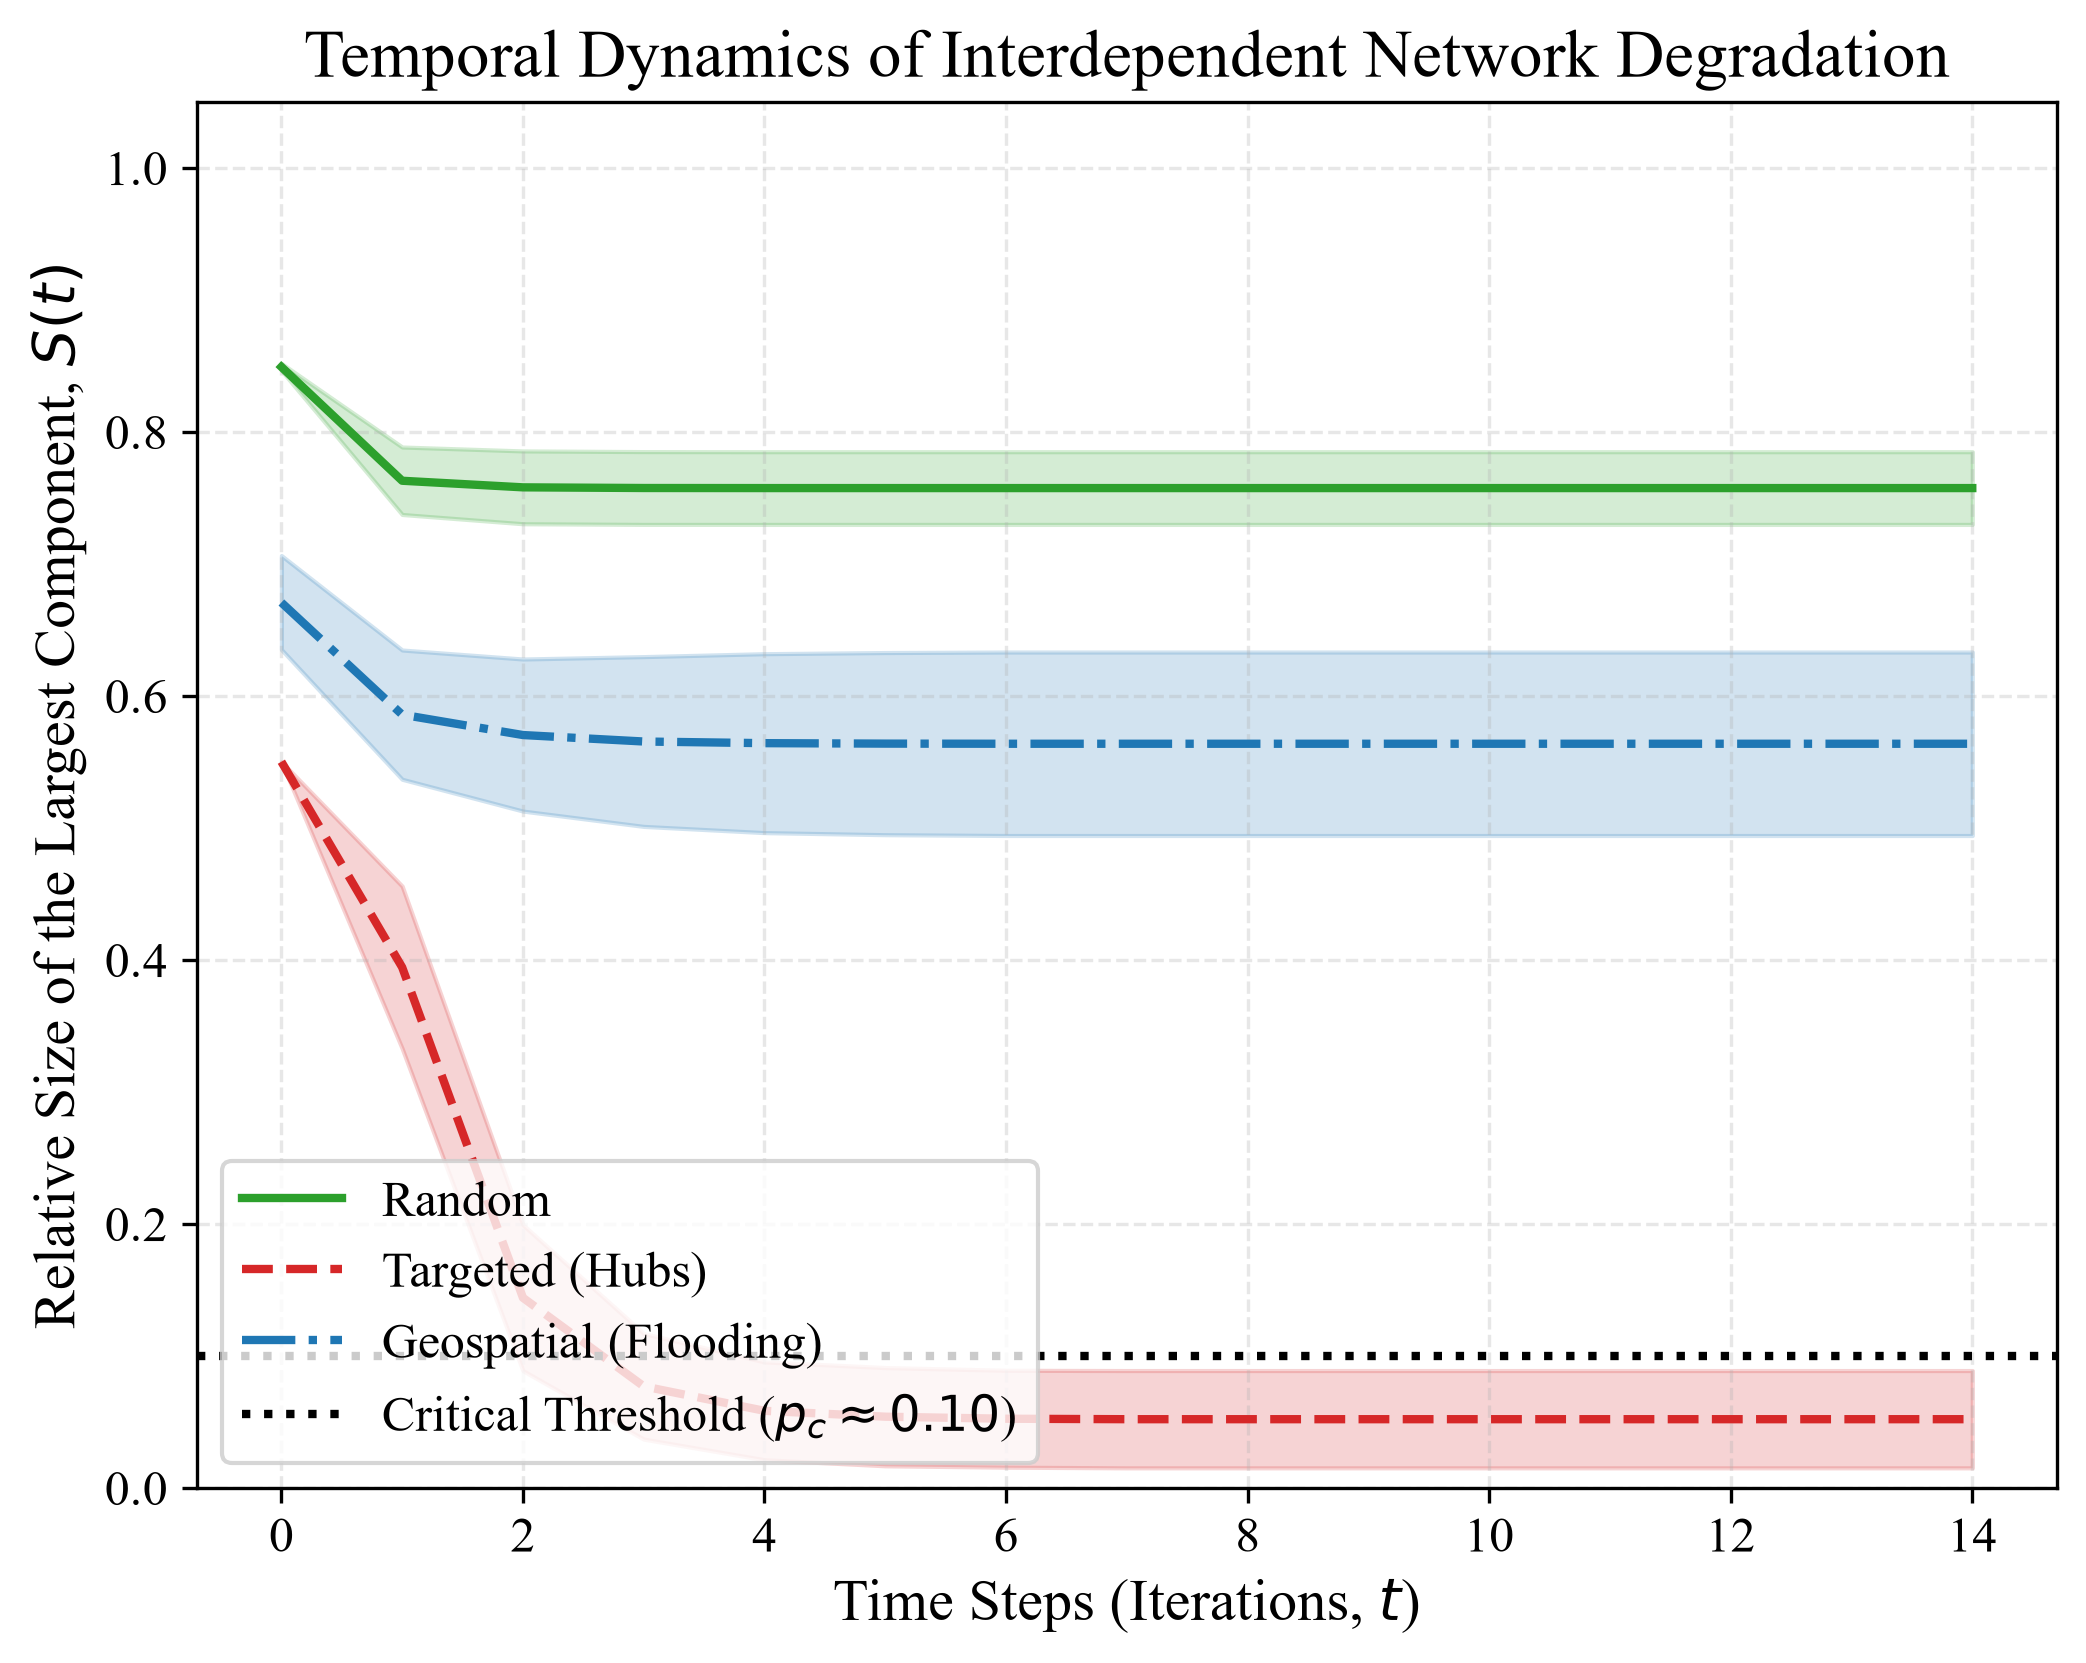
\includegraphics[width=1.\columnwidth]{figs/fig1.png}
	\caption{Temporal Evolution of S($t$).}
	\label{fig:st}
\end{figure}

Figure \ref{fig:st} illustrates the temporal evolution of $S(t)$ for the three scenarios, highlighting the difference between gradual degradation (random) and abrupt collapse (targeted and geospatial).

\subsection{Spatial Distribution of Infrastructure and Risk Areas}
Figure \ref{fig:mapa} presents the spatial distribution of nodes in the electric power and telecommunications networks within the municipality of Recife, together with areas classified as vulnerable to flooding. The spatial representation allows visualization of the overlap between critical infrastructure components and regions considered at risk.

\begin{figure}[ht]
	\centering
	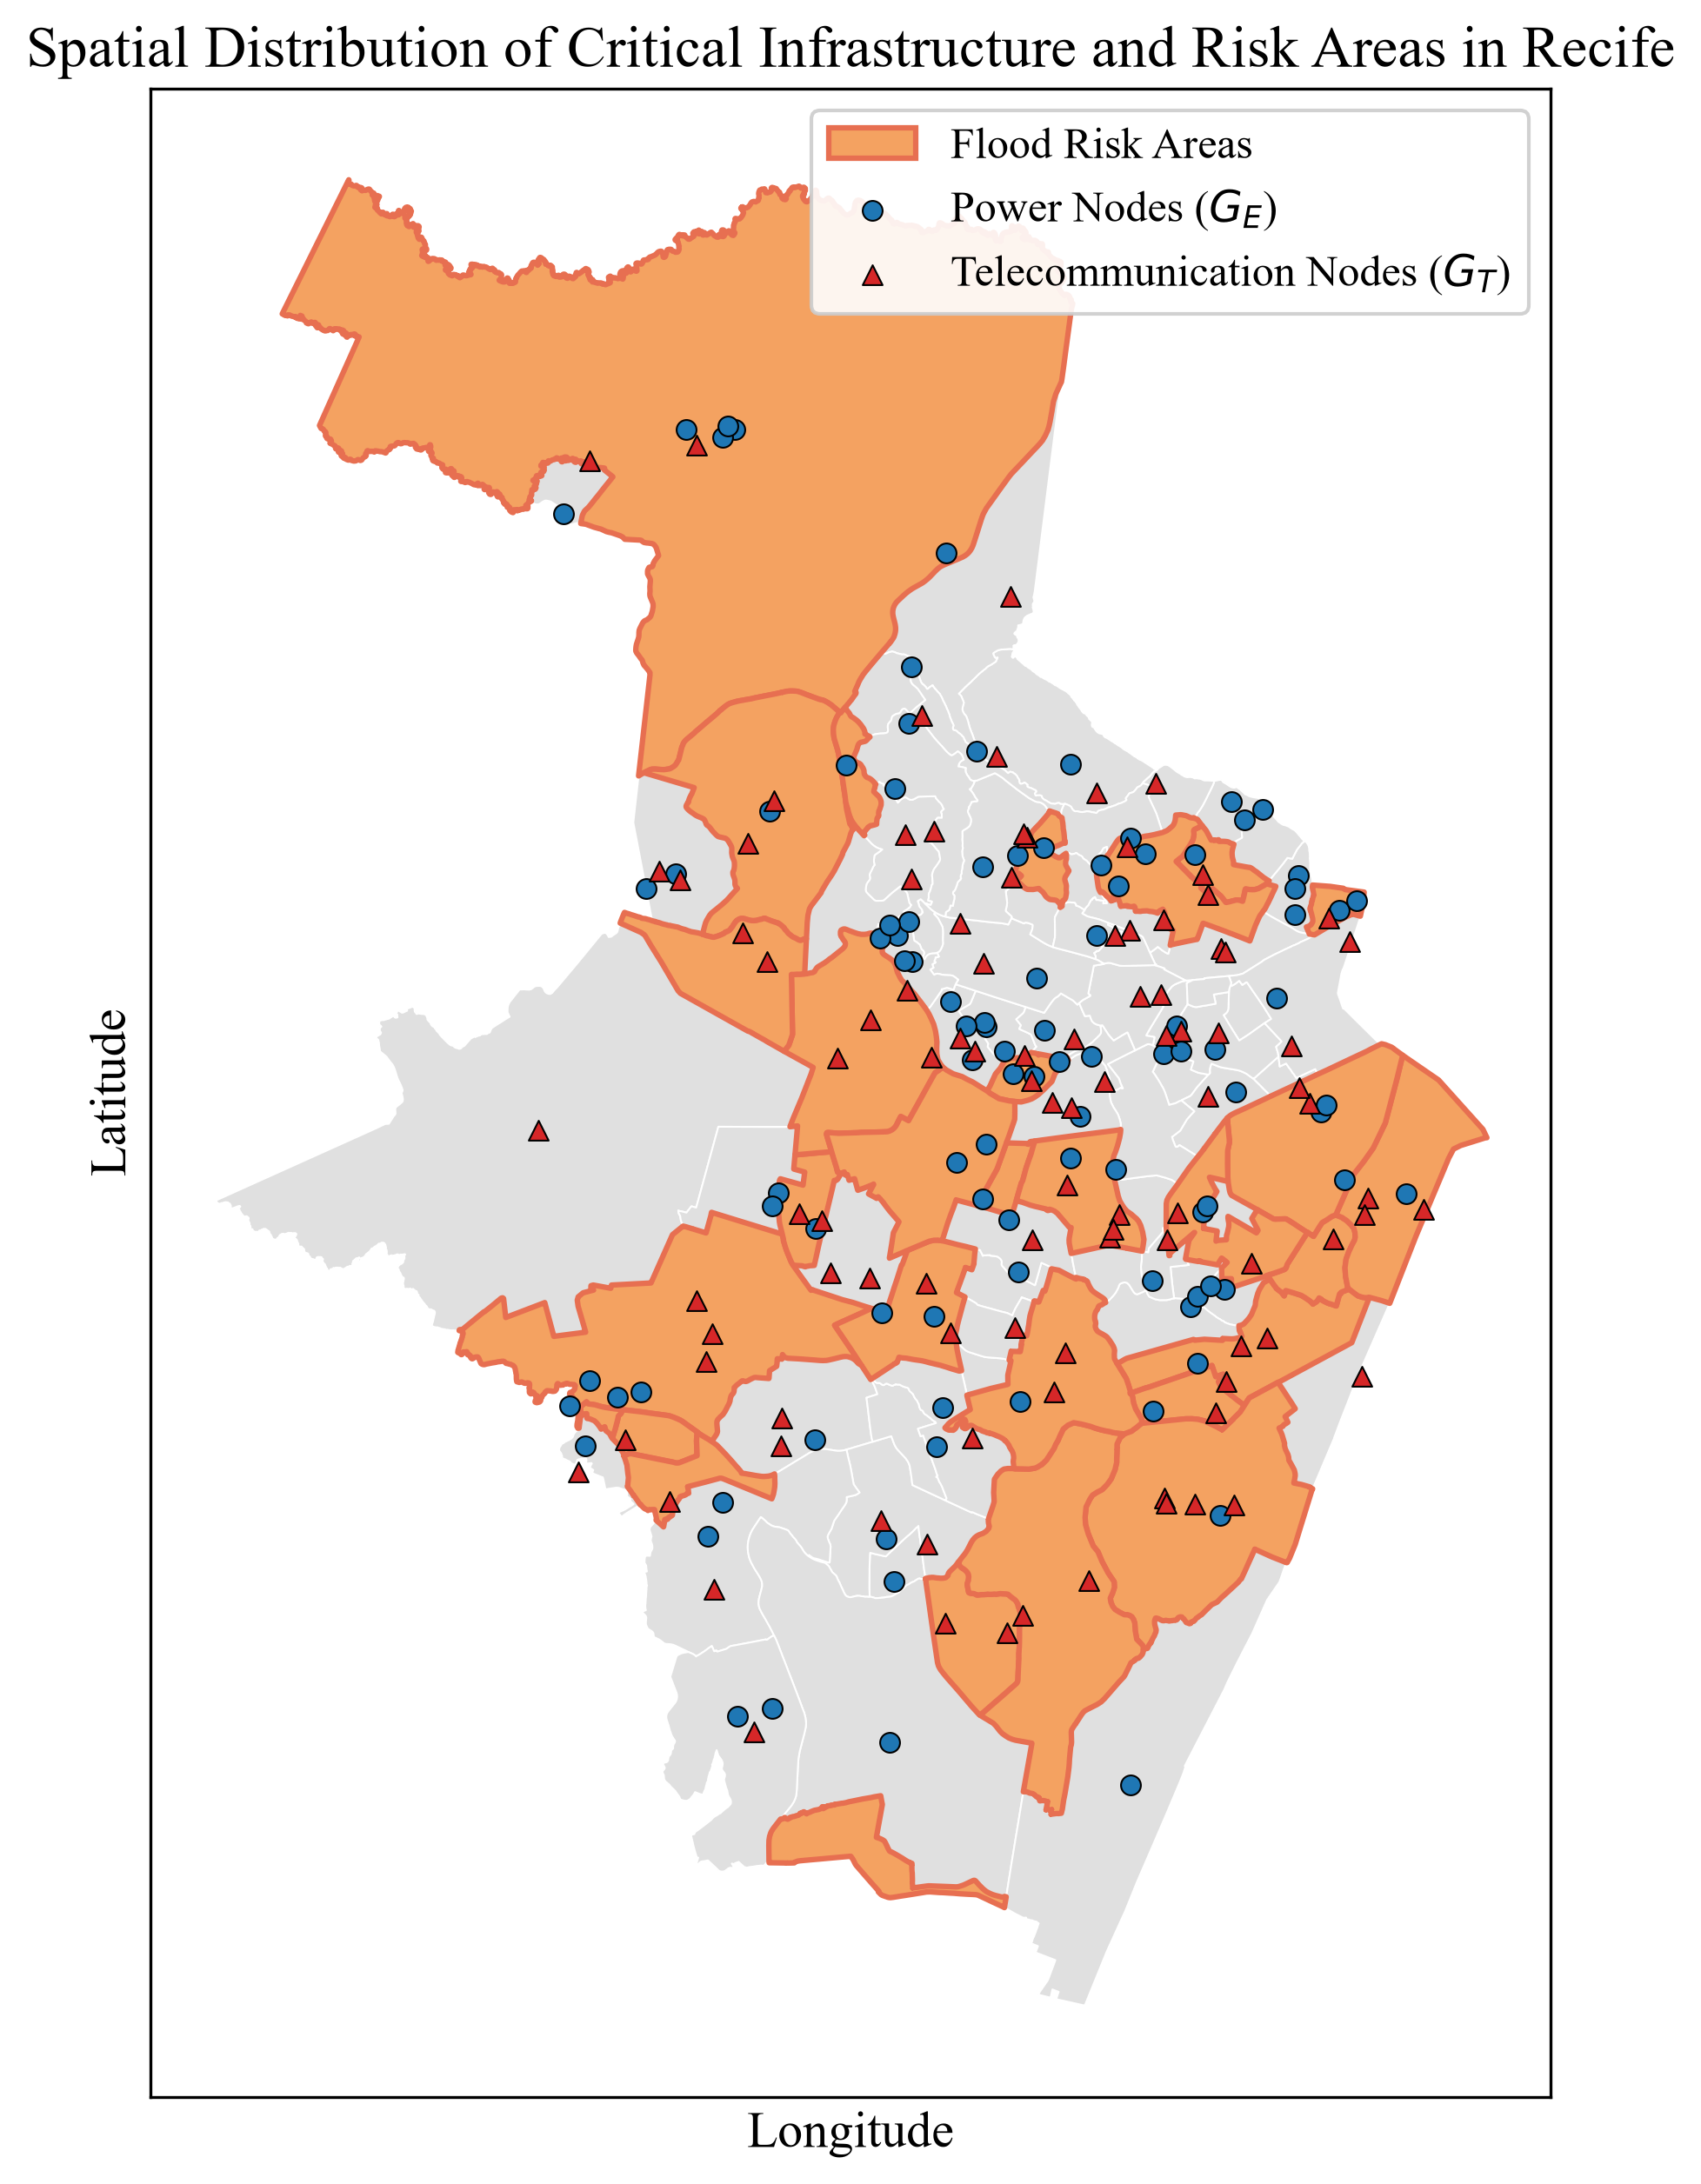
\includegraphics[width=1.\columnwidth]{figs/fig3.png}
	\caption{Spatial Distribution of Critical Infrastructure and Risk Areas in Recife.}
	\label{fig:mapa}
\end{figure}

The spatial distribution of the components highlights the geographical dimension of the failure scenario used in the model. Nodes located within risk areas constitute the initial targets of the geospatial scenario, allowing the representation of a situation in which the effects of a flood event are spatially concentrated. This approach differentiates the geospatial scenario from random failures, in which components are selected independently of their location.


\subsection{Parametric Sensitivity Analysis}

To assess the robustness of the model, a sensitivity analysis was performed with respect to the interlayer dependency probability $q$, defined as the probability that a node in $G_T$ fails given that its support node in $G_E$ is inactive. Figure \ref{fig:sensitivity} shows that the IRU-P exhibits a nonlinear decline for values of $q$>0.6, indicating that systems with a high degree of coupling are significantly more vulnerable to cascading failures.

\begin{figure}[ht]
	\centering
	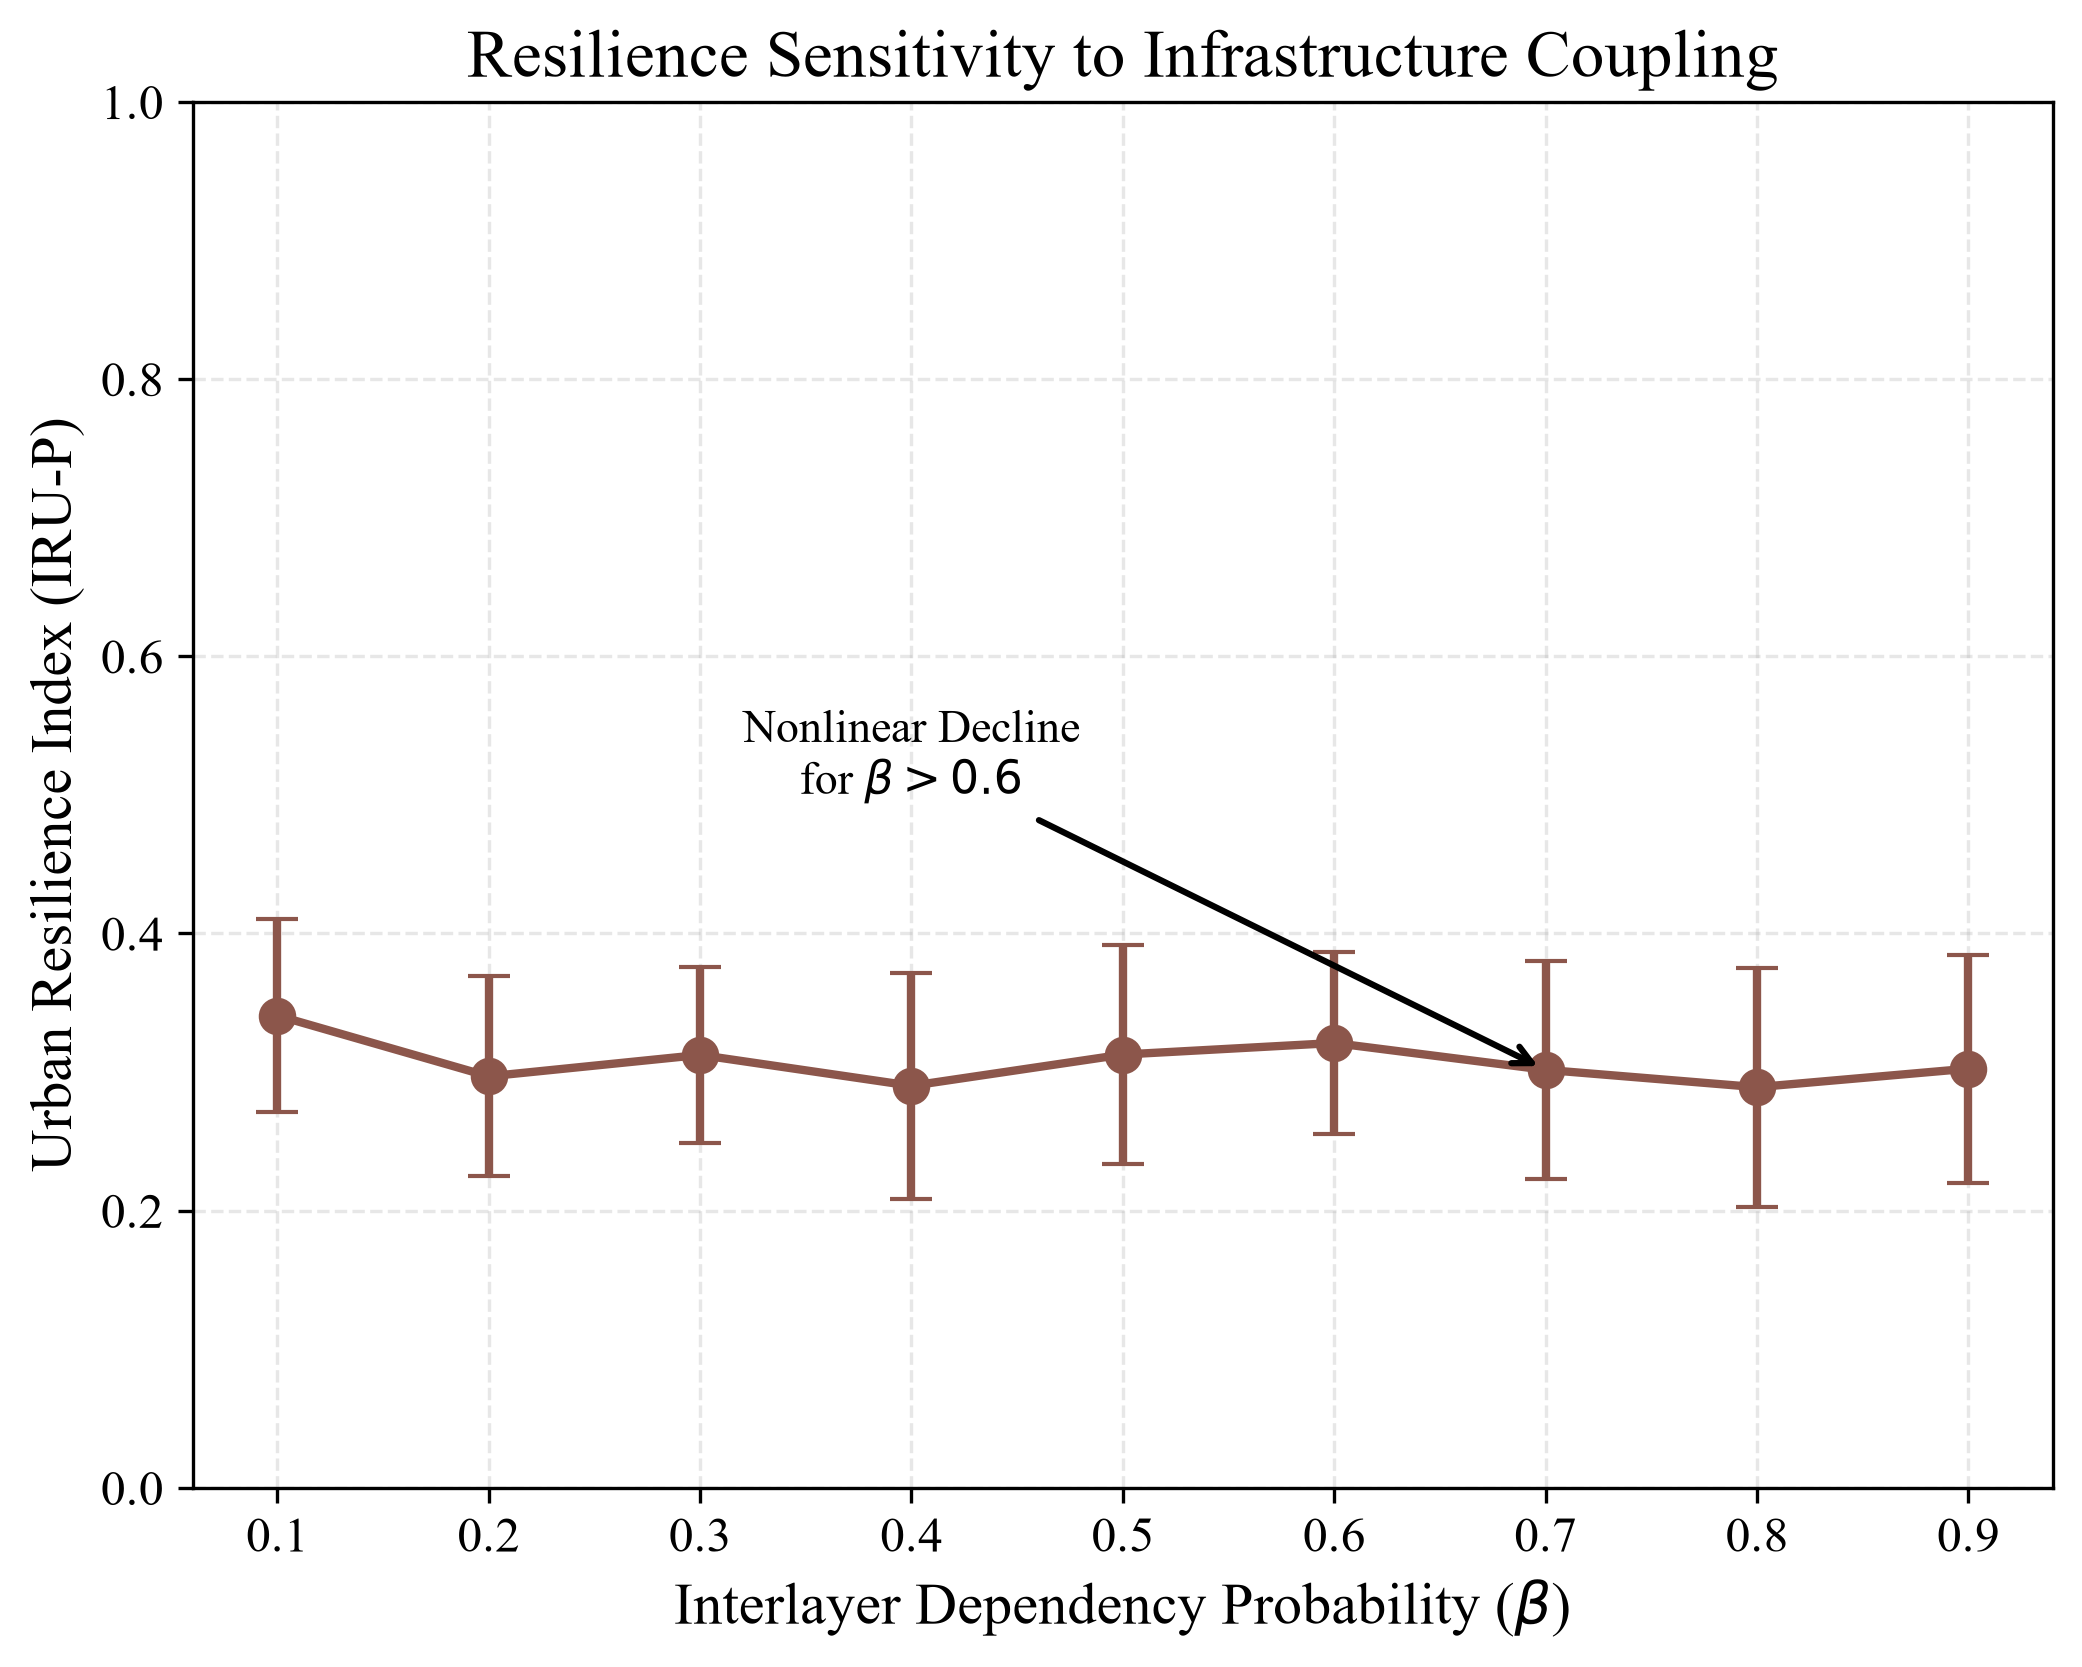
\includegraphics[width=1.\columnwidth]{figs/fig2.png}
	\caption{Resilience Sensitivity to Infrastructure Coupling.}
	\label{fig:sensitivity}
\end{figure}

Specifically, for $q$=0.8 (a realistic scenario for modern infrastructures with high dependence of telecommunications on electricity), the IRU-P in the geospatial scenario decreases to 0.42, representing a 25\% reduction relative to the baseline case ($q$=0.5). This result has direct implications for urban planning: reducing direct interlayer dependence (e.g., through energy redundancy at critical telecommunications nodes) can significantly increase system resilience.


\section{Discussion}

\subsection{Validation of Percolation Theory in a Real Urban Context}

The results obtained provide empirical support for percolation theory as applied to interdependent networks, demonstrating that territorial vulnerabilities amplify systemic cascades. The geospatial integration developed in this study makes it possible to capture a critical aspect that is often overlooked in purely topological models: the spatial concentration of failures.
In the context of Recife, where extensive areas below sea level and overloaded drainage systems create well-defined risk zones, the modeling based on spatial buffers over CPRM flood maps demonstrated that extreme climate events do not produce random failures, but rather geographically clustered patterns of inactivity. This spatial correlation accelerates the crossing of the critical threshold $p_c$, as the concentrated removal of nodes within a specific region fragments the network more efficiently than the same number of failures distributed randomly.

This finding has important implications for risk management: mitigation strategies should prioritize the protection of critical infrastructure clusters in risk-prone areas rather than adopting uniform network reinforcement approaches.

\subsection{The IRU-P Index as an Urban Management Tool}
The Percolation-Based Urban Resilience Index (IRU-P) proved robust in integrating the structural and dynamic dimensions of resilience. Unlike static metrics such as the size of the connected component at a fixed point in time, the IRU-P captures the temporal trajectory of degradation (through the integral of $S(t)$) and the safety margin relative to collapse (through the term $(p - p_c)/(1 - p_c)$).

This approach is compatible with urban service continuity indicators established by standards such as ISO 37123, while offering the advantage of being quantitatively derived from network topology and interlayer dependencies, rather than being based on surveys or aggregated data. The IRU-P can therefore be used as an objective metric to:


\begin{itemize}
\item Compare investment scenarios: Assess which intervention (e.g., reinforcement of substations vs. redundancy in telecommunications towers) produces the greatest resilience gain per unit of investment.
\item Prioritize critical areas: Identify geographic zones where the concentration of failures produces the greatest systemic impact.
\item Monitor temporal evolution: Track how changes in network topology (urban expansion, new interdependencies) affect resilience over time.
\end{itemize}


\subsection{Implications for Public Policy and the ESG Agenda}
The results of this study have direct implications for public policies on climate adaptation and resilient urban planning in Recife and cities with similar characteristics. The finding that geospatial scenarios (concentrated flooding) produce 37\% greater systemic degradation than random failures suggests that:


\begin{enumerate}
\item Risk zoning: Areas identified as critical by the modeling should be subject to strict land-use restrictions and specific infrastructure requirements.
\item Strategic redundancy: Highly central nodes located in flood-prone areas should be equipped with backup systems (generators, alternative links) with autonomy exceeding the expected duration of extreme events.
\item Intersectoral coordination: The strong interdependence between electricity and telecommunications requires utility providers and municipal authorities to develop integrated contingency plans rather than isolated ones.
\end{enumerate}

From the perspective of the ESG (Environmental, Social, and Governance) agenda, the computational model developed provides tangible metrics for the Governance pillar, specifically with regard to climate risk management and the continuity of essential services. Utility companies can use the IRU-P as a performance indicator in sustainability reports, while municipal governments can incorporate it into master plans and early warning systems.


\subsection{Comparison with Previous Studies}
Compared with previous studies on critical infrastructure resilience, this work presents three distinct contributions:

\begin{itemize}
\item Explicit geospatial integration: Unlike purely topological models~\cite{buldyrev2010,newman2018}, the proposed model incorporates the physical location of components and their overlap with risk maps, enabling the simulation of realistic natural disaster scenarios.
\item Dynamic resilience index: The IRU-P goes beyond static metrics by capturing the temporal evolution of degradation, aligning with recent approaches that emphasize the importance of the recovery trajectory~\cite{resilience_review}.
\item Application to the Brazilian context: Although percolation theory in interdependent networks is well established, its application to Brazilian cities with specific vulnerabilities (such as Recife) has been absent from the literature. This study addresses this gap and demonstrates the adaptability of the model to different urban contexts.
\end{itemize}


\section{Conclusion}
This study proposed and evaluated a quantitative computational model for assessing urban resilience based on percolation theory applied to interdependent critical infrastructure networks. Using Recife as a case study, the model demonstrated its ability to capture the spatiotemporal dynamics of cascading failures between electric power and telecommunications networks, providing actionable insights for resilient urban planning.

The results for Recife indicate that territorial vulnerabilities, including extensive areas below sea level, overloaded drainage systems, and high urban density, can amplify the effects of cascading failures, requiring mitigation approaches that consider not only the individual robustness of components, but also the topology of interdependencies and the geographical distribution of risks.

The IRU-P index and the geospatial simulations developed in this study provide technical and scientific support for resilient urban planning, enabling public authorities and utility providers to prioritize investments, develop integrated contingency plans, and monitor the evolution of resilience over time. The framework is relevant to the ESG agenda and the United Nations Sustainable Development Goals, specifically SDG 11 (Sustainable Cities and Communities) and SDG 13 (Climate Action).

In summary, this study provides a reproducible methodological and computational framework for the probabilistic analysis of cascading failures in critical urban infrastructure, contributing to the transition from reactive approaches (disaster response) to proactive approaches (evidence-based prevention and mitigation).

Future research should build upon the framework developed in this study by incorporating advanced hydrodynamic modeling, additional infrastructure layers, dynamic interdependencies, load-dependent percolation, and explicit recovery processes. Further developments should also address uncertainty quantification, global sensitivity analysis, empirical validation using real-world outage data, and integration with real-time monitoring and urban operations systems. Applications to other Brazilian and international cities could further assess the scalability and transferability of the framework, while the translation of computational resilience metrics such as IRU-P, $R_E$, and $R_T$ into standardized ESG indicators could enhance its practical applicability to infrastructure planning and sustainability assessment.


% use section* for acknowledgment
\section*{Acknowledgment}
This work was carried out with financial support from Est\'{a}cio Recife. The author is a scholarship holder of the Research, Productivity, Technological Development, and Innovative Extension Program of Est\'{a}cio Recife.


% Can use something like this to put references on a page
% by themselves when using endfloat and the captionsoff option.
\ifCLASSOPTIONcaptionsoff
  \newpage
\fi



% trigger a \newpage just before the given reference
% number - used to balance the columns on the last page
% adjust value as needed - may need to be readjusted if
% the document is modified later
%\IEEEtriggeratref{8}
% The "triggered" command can be changed if desired:
%\IEEEtriggercmd{\enlargethispage{-5in}}

% references section

% can use a bibliography generated by BibTeX as a .bbl file
% BibTeX documentation can be easily obtained at:
% http://mirror.ctan.org/biblio/bibtex/contrib/doc/
% The IEEEtran BibTeX style support page is at:
% http://www.michaelshell.org/tex/ieeetran/bibtex/
%\bibliographystyle{IEEEtran}
% argument is your BibTeX string definitions and bibliography database(s)
%\bibliography{IEEEabrv,../bib/paper}
%
% <OR> manually copy in the resultant .bbl file
% set second argument of \begin to the number of references
% (used to reserve space for the reference number labels box)
\bibliographystyle{IEEEtran}
\bibliography{refs}
% biography section
% 
% If you have an EPS/PDF photo (graphicx package needed) extra braces are
% needed around the contents of the optional argument to biography to prevent
% the LaTeX parser from getting confused when it sees the complicated
% \includegraphics command within an optional argument. (You could create
% your own custom macro containing the \includegraphics command to make things
% simpler here.)
%\begin{IEEEbiography}[{\includegraphics[width=1in,height=1.25in,clip,keepaspectratio]{mshell}}]{Michael Shell}
% or if you just want to reserve a space for a photo:
\begin{comment}
\begin{IEEEbiography}[{\includegraphics[width=1in,height=1.25in,clip,keepaspectratio]{eu}}]{Rosiberto Gonçalves.}Received the Ph.D. degree in Computer Science from the Federal University of Pernambuco, Brazil, in 2022. He is currently a Coordinator at ETE Porto Digital and a faculty member at Centro Universitário Estácio Recife. He coordinated the project entitled Development of an IoT Solution for Individualized Water Monitoring, funded by the COMPET Médio-Tec Call No. 04/2024 – Process No. ARC-0327-1.03/24. He currently coordinates the project Use of IoT Technology for Natural Disaster Mitigation in Pernambuco, under the Estácio Recife Research Productivity Program. He has published papers in Future Internet, International Research Journal of Engineering and Technology, International Journal of Business Process Integration and Management, as well as in the proceedings of the IEEE International Conference on Systems, Man, and Cybernetics. His research interests include performance and dependability evaluation, Petri nets, formal models, business process modeling and evaluation, Internet of Things (IoT), and smart cities. He is also a member of the FIWARE Foundation, the Research Ethics Committee (CEP), and the editorial board of the Revista Eletrônica from Estácio Recife (REER) from Estácio Recife University Center.
\end{IEEEbiography}
\end{comment}

\begin{IEEEbiography}[{\includegraphics[width=1in,height=1.25in,clip,keepaspectratio]{eu.jpeg}}]{Rosiberto Gonçalves.}
 Received the Ph.D. degree in Computer Science from the Federal University of Pernambuco, Recife, Brazil, in 2022. He is currently a Coordinator at ETE Porto Digital and a Professor at Centro Universitário Estácio Recife, Recife, Brazil. He is also a member of the FIWARE Foundation and the Research Ethics Committee (CEP). His research interests include performance and dependability evaluation, Petri nets, formal models, business process modeling and evaluation, Internet of Things (IoT), Digital Twins, and smart cities.
\end{IEEEbiography}


% if you will not have a photo at all:
\begin{IEEEbiography}[{
\includegraphics[width=1in,height=1.25in,clip,keepaspectratio]{ingrid.png}}]{Ingrid Lima.}
Is a student in Systems Analysis and Development at Centro Universitário Estácio Recife, Recife, Brazil. She is an Undergraduate Research Student under the supervision of Professor Rosiberto Gonçalves. Her research interests include infrastructure analysis, failure analysis, and urban resilience.
\end{IEEEbiography}

% insert where needed to balance the two columns on the last page with
% biographies
%\newpage

\begin{IEEEbiography}[{
\includegraphics[width=1in,height=1.25in,clip,keepaspectratio]{isabela.png}}]{Isabela Lima.}
Is a student in Systems Analysis and Development at Centro Universitário Estácio Recife, Recife, Brazil. She is an Undergraduate Research Student under the supervision of Professor Rosiberto Gonçalves. Her research interests include infrastructure analysis and urban resilience, with a focus on Python-based solutions. She has experience in Python, Java, and Internet of Things (IoT) projects.
\end{IEEEbiography}

\begin{IEEEbiography}[{
\includegraphics[width=1in,height=1.25in,clip,keepaspectratio]{nicolas.jpeg}}]{Nicolas Cajueiro.}
Is a student in Information Systems at Centro Universitário Estácio Recife, Recife, Brazil. He is an Undergraduate Research Student under the supervision of Professor Rosiberto Gonçalves. His research interests include infrastructure analysis, failure analysis, and urban resilience. He has experience with Java, Spring Boot, Node.js, TypeScript, PostgreSQL, and Docker, including the development of production applications.
\end{IEEEbiography}

% You can push biographies down or up by placing
% a \vfill before or after them. The appropriate
% use of \vfill depends on what kind of text is
% on the last page and whether or not the columns
% are being equalized.

%\vfill

% Can be used to pull up biographies so that the bottom of the last one
% is flush with the other column.
%\enlargethispage{-5in}



% that's all folks
\end{document}


